\documentclass{article}
\usepackage{CJK}
\usepackage{CJKulem}
\usepackage{indentfirst}
\usepackage{graphicx}
\begin{CJK}{UTF8}{song}
\title{深度学习防骗指南}
\author{戚锦秀}
\date{\today}
\begin{document}
\maketitle

\begin{abstract}
毕业于哈尔滨工业大学控制科学工程系,目前担任金融事业部数据挖掘工程师,负责数据仓库开发,用户画像构建,信贷数据建模,神经病画风的码农。
\end{abstract}

机器学习圈子里有三大灌水神器:图模型加圈,神经网加层,准则函数加正则。今天主要讨论的是神经网加层这块,别紧张,这篇文章基本不会出现数学公式,需要用到数学公式的地方我会把它转化成非专业人员也能听懂的话来描述。既然叫防骗指南,那又如何保证这篇文章不是一个骗局呢?这个问题三百年前休谟就回答过了,“除了我之外在场的所有人说的话都不靠谱”。不过你依然需要怀着怀疑的心态看这篇文章,毕竟我也经常挖坑给自己跳。



\section{Deep Learning}
这几年深度学习的概念很火,出门打招呼不扯两句深度学习都不好意思说自己是搞数据的。在大众眼里,我们似乎在仿生大脑,人工智能威胁论是吧,奇点临近是吧;在工程师眼中,我们好像能赚很多钱,打断双腿都不用愁下半生;然而在数学家眼里的我们不过是在玩泥沙渣渣,毕竟我们连个像样的误差界都证不出;当然咯,他们的看法并不妨碍我们自己眼中西小口/海淀吴彦祖的形象;但事实上呢?我们每天都在干什么呢?我们每天就在中关村步行街上搭个摊子,吆喝着“祖传调参,五元一层嘞”

\begin{center}
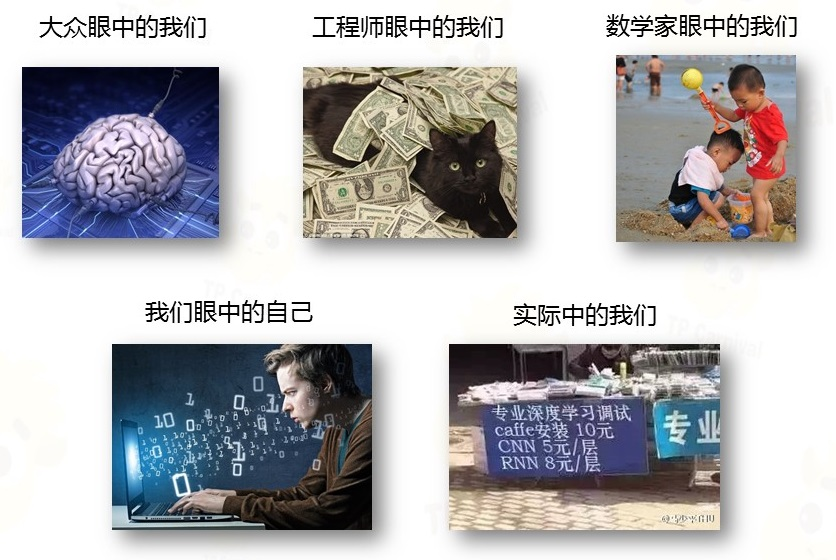
\includegraphics[width=3.5in]{image/image5.jpg}
\end{center}


那么什么是深度学习?深度学习,说到底不外乎是一系列深层的神经网络,而这一系列的神经网络根据不同的假设又会有不同的构型,为了说清楚什么是深度学习,我们先要解决一个问题:什么是神经网络。
\subsection{What is Neural Networks?}




大部分学过机器学习的人接触的第一个模型都是Logistic回归,其实Logistic回归就是一种最简单的神经网络,我们有d个输入,1,2,3,blabla 一直到d,比如$x_1$是机票订单数,$x_2$是酒店订单数等等。这些特征乘上对应的参数$w_1$, $w_2$ blabla,简单又粗暴地,你可以把它理解为特征的重要性,然后一相乘再相加,就得到了一个实数,也就是这里的$wx$,最后一个非线性映射映射,啪的一声,一个神经元就激活了,这个节点的输出就可以预测你会不会借钱不还,你在下个月能不能脱离单身狗苦海。一个单节点的神经网络就这么出现了。

\begin{center}
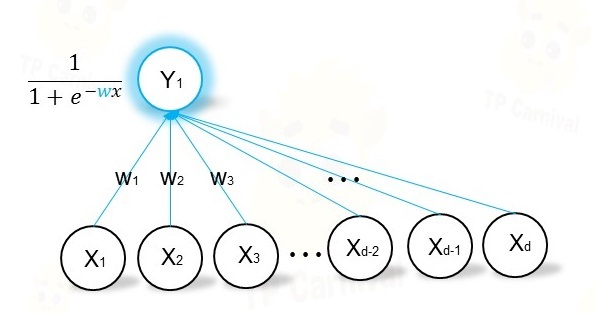
\includegraphics[width=2.5in]{image/image7.jpg}
\end{center}


好,与刚刚的过程类似,啪的一声,我们又加了一个绿色的神经元。
\begin{center}
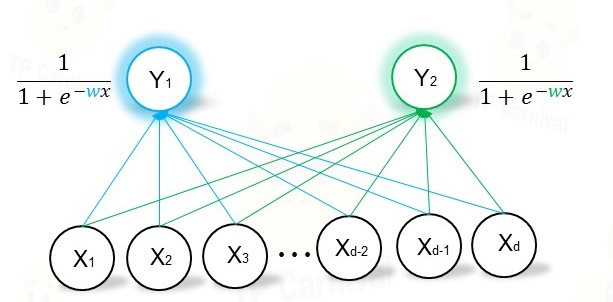
\includegraphics[width=2.5in]{image/image8.jpg}
\end{center}


再啪的一下,我们又加了一个红色的神经元,当然咯,我们可以在这一层加任意多的神经元,你看,我们这几个省略号不是白画的嘛。

\begin{center}
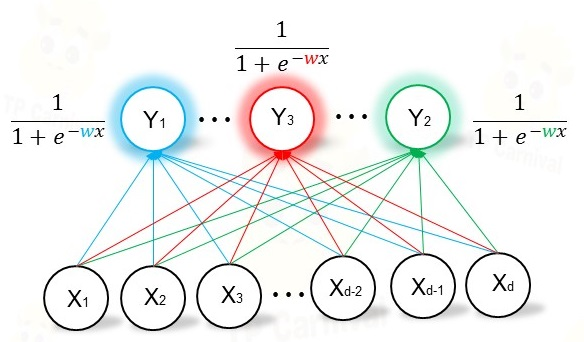
\includegraphics[width=2.5in]{image/image9.jpg}
\end{center}

聪明的同学已经能想到了,我们接下来要加层了,没错,在红绿蓝的基础上,我们在上面加了一青一黄两个神经元,分别代表一个用户会还钱,以及不会还钱,作为模型的输出。


\begin{center}

\includegraphics[width=3in]{image/image10.jpg}
\end{center}


假设现在来了一个用户,我们能获取他的历史订单信息,也就是说,$x_1$ $x_2$, blabla $x_d$ 这些最底层的神经元我们是知道的,我们需要预测他会不会欠钱不还。整个预测过程是这样的,数据从最底层注入到中间层,也就是红蓝绿这层,这层我们也叫作特征层提取层,然后在注入到最顶层的输出层,输出的值作为你的预测值。


但是这里会有个bug,似乎我们预先就知道权值是多少,权值是哪来的?产品经理定的?还是谁定的?如果说处于冷启动状态,也就是你没有训练样本,那么一般都是由专家赋权(不过这时候基本不会使用神经网络而是别的模型)。一旦你积累了一定量的数据,你就可以通过训练样本来确定这些权值,也就是我们经常说的“让数据发声”。

怎么训练得到权值?

\begin{quote}
没有什么是抛一次硬币解决不了的,如果有,那就两次。

\rightline{---蒙特卡洛}
\end{quote}

既然没有什么比抛硬币更好,那不妨初始化的时候就随机设置权值好了,然后通过样本来对权值进行迭代的修正,什么个意思呢?不妨举个例子。

假设三胖造了些导弹想要扔到民主灯塔去,因为第一次扔嘛,没啥经验,能力也不强,就随便扔好了,结果一不小心扔到南极去了,这时候企鹅爸爸就出来发言了“你也不想想,不充钱你会变强吗?”于是三胖充了个会员,企鹅爸爸就告诉他“你刚刚啊,太用力了,太用力知道吗?都跑到南半球了,你别那么使劲,明白?”这次三胖长记性了,轻一点,一不小心就把某猪场炸了,养猪大户就跑出来喷了,“方向!方向不对!你瞄准点行不行!”。

所谓模型的训练,就跟上面这个过程类似。一开始随机碰运气,碰壁了后老师告诉你应该怎样怎样,每一次碰壁就是一个训练样本,每次碰壁后的老师就是样本的标签,随着碰壁的次数不断增多,模型的精度就会上升(当然不会无限上升,不然我做完所有的五年高考三年模拟岂不是就能考上蓝翔了?)


\subsection{Why was the BP named BP ?}
我们都知道,神经网络的第二次兴起的一个重要原因是八十年代BP算法的提出。我认识不少朋友,他们推导得了链式求导,却不一定能解释为什么它叫做反向传播,这里,我们会解释一下,反向传播为什么取名为反向传播,而不是别的名字。

一个神经网络,其原始数据经过多层隐含层的传播,到达最顶层的输出层,这时候会与标签,即教师信号做比较,各个节点自然就会有误差,这个误差反向注入(注意我用的是注入这个词而不是传播这个词,因为注入会更形象)回上一层,就像你前向传播的过程一样,而上一层神经元接收到这个误差后,修正自身这一层的权值,然后计算这一层的误差,再将这层的误差继续反向注入到它的再前一层。这就是反向传播中链式求导的非数学语言描述。

\begin{center}
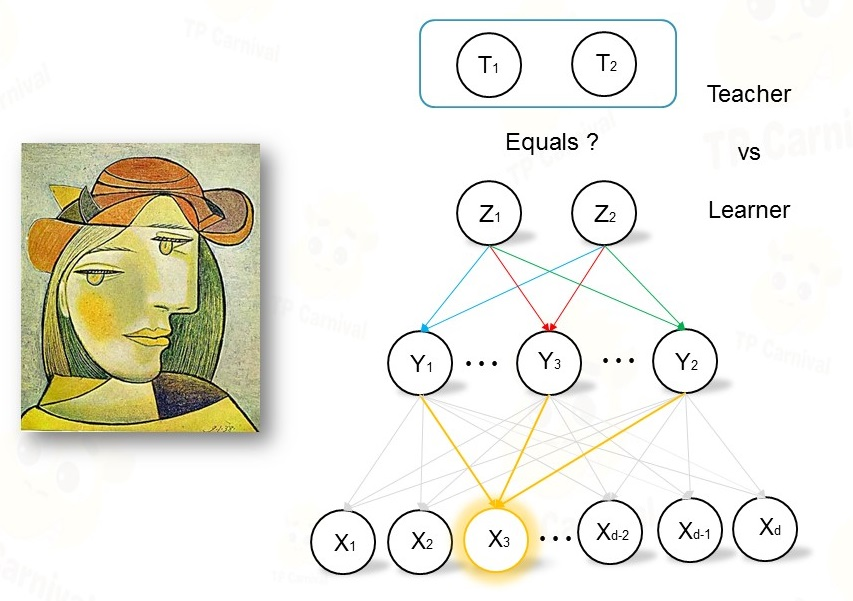
\includegraphics[width=4in]{image/image100.jpg}
\end{center}

就好比你去看毕加索的画,你会十分困惑,“咦?你这长得不大对啊,怎么左眼的隔壁,还有一个左眼呢?”,抛开艺术层面,如果我们要修正毕加索的画,使得它看起来像个正常人,怎么办?首先,你先把眼睛的位置修正好,眼睛的位置一旦修正了,鼻子的误差是不是就可以知道了啊?然后你修正鼻子后,嘴巴的误差是不是就可以知道了?反向传播就像是这样一个过程,权值修正的时候,由最顶层开始,一边反向注入一边修正权值,直至到将最开始的那层权值修正完毕。

反向传播看起来似乎很美好,但当你使用卷积网络的时候就不那么优雅了,因为会涉及kron积以及卷积自相关的性质,而在RNN就会涉及到展开问题,你要是说现在你还手工写反向传播,那我敬你是条汉子。现在的计算框架基本都是走自动梯度而不是反向传播了(当然,反向传播是自动梯度的一个特例),也就是说,你只需要定义前向传播,梯度由计算框架自动帮你计算。本来想写一下自动梯度原理的,但是管理员催稿,所以就跳过咯。




\subsection{Step by setp, stack by stack}
上面我们只是建了三层网络,有的同学可能就会不服了,“我当了24年单身狗,就不允许我建24层网络?”“我追随长者这么多年,90大寿建一个90层网络不行?”,啊,这几位同学,你们很有前途,你们的讨论其实就是深度学习的范畴了,我这里有本《深度学习调参指南》,10块两本10块两本。

我们先介绍第一种深度结构,不妨叫做encoder结构好了,有时候我们也就叫他自编码机。首先我们有一层输入

\begin{center}
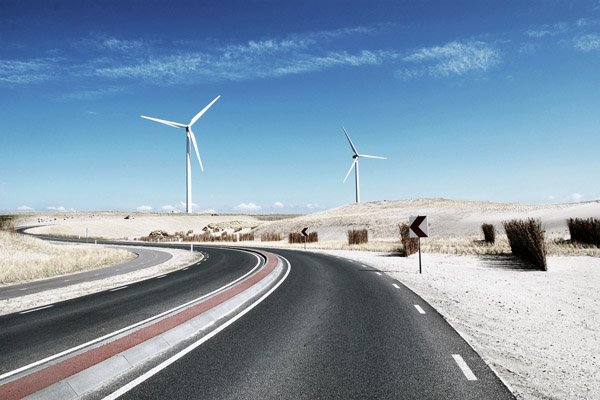
\includegraphics[width=1.1in]{image/image12.jpg}
\end{center}

然后我们从这层输入中提取了一些特征,这个过程叫做编码

\begin{center}
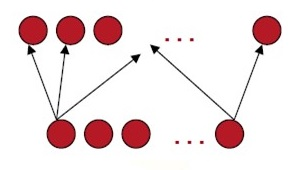
\includegraphics[width=1.1in]{image/image13.jpg}
\end{center}

这些特征好不好啊?如果说这些特征能还原回原始数据,那么我们就认为这些特征学到关键点上了。所以,说我们让特征层的上一层,也就是蓝色的神经元,以原始数据为学习目标,试图将它还原回去,这个过程叫做解码。

\begin{center}
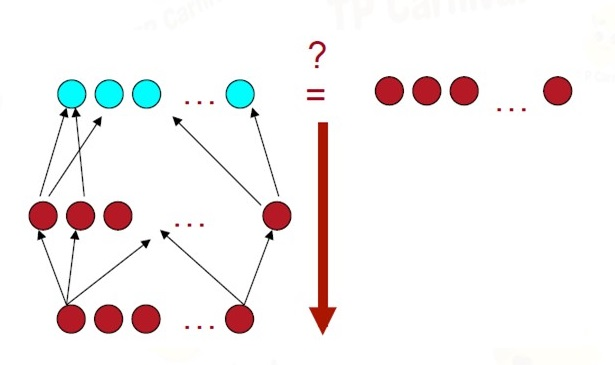
\includegraphics[width=2in]{image/image14.jpg}
\end{center}

当这个网络学习完后,我们就会cut掉蓝色的神经元,这是就得到了一个编码机。

\begin{center}
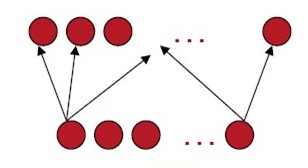
\includegraphics[width=1.1in]{image/image15.jpg}
\end{center}

接着我们在此基础上再做一次编码

\begin{center}
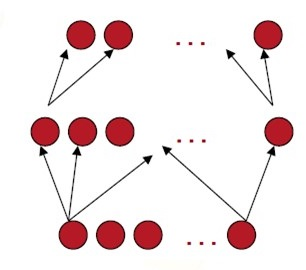
\includegraphics[width=1.1in]{image/image16.jpg}
\end{center}


然后还原
\begin{center}
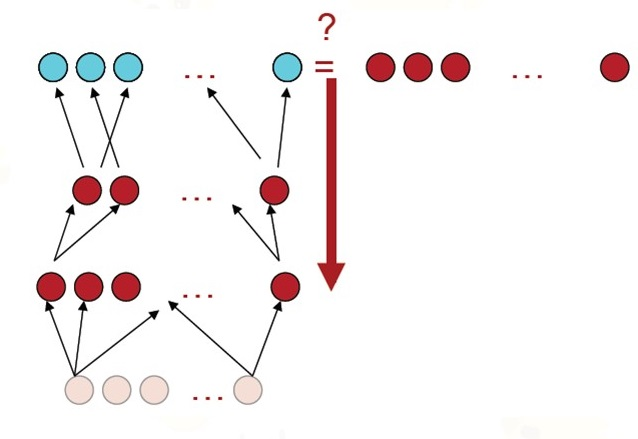
\includegraphics[width=2.2in]{image/image17.jpg}
\end{center}
然后cut掉蓝色神经元

\begin{center}
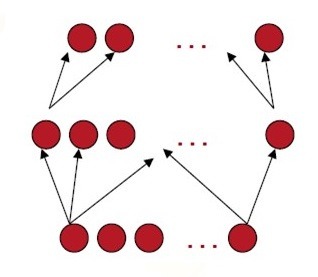
\includegraphics[width=1.2in]{image/image18.jpg}
\end{center}

以此类推,你再加一层

\begin{center}
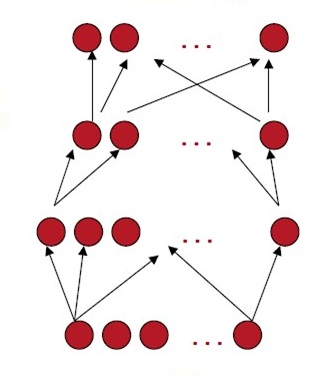
\includegraphics[width=1.2in]{image/image19.jpg}
\end{center}

诶,再加一层

\begin{center}
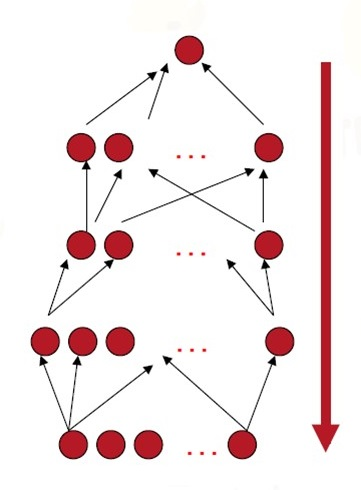
\includegraphics[width=1.2in]{image/image20.jpg}
\end{center}

好了5层的神经网络就这么建起来了,这个过程,我们称作无监督的预训练,他的目标仅仅是为了学会重构自己。所以,在分类任务中,你还需要一次有监督的反向传播微调。


编码机的核心思想就是这些,他就好像是一个随动系统,不断的跟踪系统的输入,将其复现出来。不同的编码机只是一些细节上的差异,比如,如果希望稀疏表达,那么就在准则函数加KL散度;如果噪声中还原的数据,那么就在data那里加噪声;如果希望正则化准则函数,那么就在error那里加范数;如果希望模型抗干扰,那么就在error那里加雅各比矩阵,RBM比较特殊,他在数学推导上不是encoder,但他结果上也是一种基于重构的模型,所以我们也把他并入到这里了。

\begin{center}
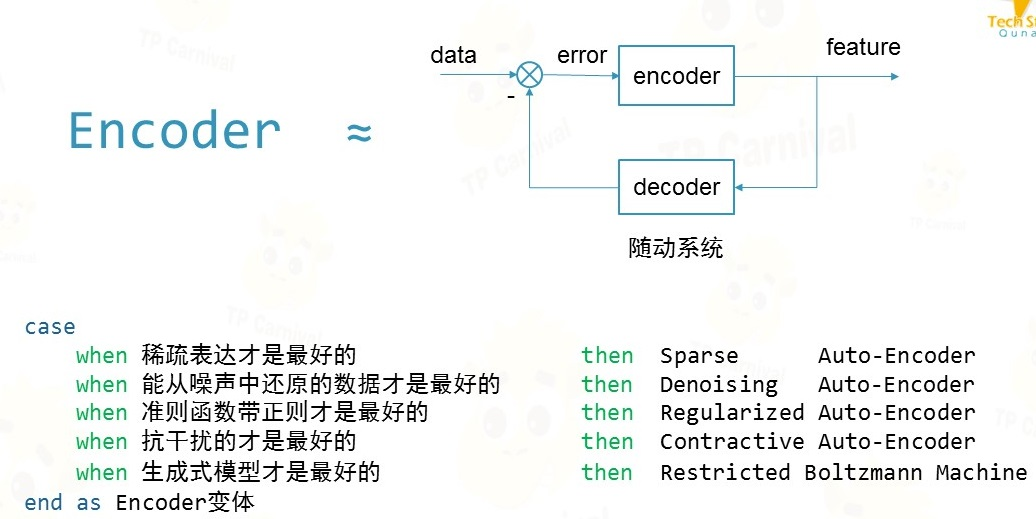
\includegraphics[width=4.5in]{image/image21.jpg}
\end{center}


所谓正则,不过是你对一些参数的先验罢了,个人认为正则化是为了防止过拟合这种说法是不太对的。你可以在准则函数上加上任何你期望的罚函数,比如你知道某个参数wi不可能为负,那完全可以加一个error +(-wi)啥的,有些人可能会反驳我,准则函数加上二范数后确实能避免过拟合啊,没错,大多数情况下确实如此,但为什么可以防治过拟合呢?因为发生过拟合的时候,权值一般都会偏大(参考PRML的讨论),这也就解释了神经网络中为什么会有权衰减(其实等价于准则函数加二范数)这东西,你加上二范数后,相当于强制权值是一个比较小的数,这其实就是你的先验知识,你偏爱小权值而不是大权值。这里不展开了,再展开就到机器学习另一个灌水领域了。

当然,这里的控制框图只是不严谨的框图,真正意义上披着机器学习外衣的控制论,它的名字叫做强化学习,这又是另一个大坑,我们就别挖了吧,毕竟再挖一会地基都要塌了。




为什么深度神经网络中会采用这种无监督的预训练呢?其实无监督的预训练就像是:咦?这两个东西长得好像啊,虽然我不知道它们是什么,但我不妨先把他们放到一块吧。等到有监督的训练的时候,我告诉你这东西叫做说数字3,那么你就会推断说,哦,原来长成这样的东西叫做3。
\begin{center}
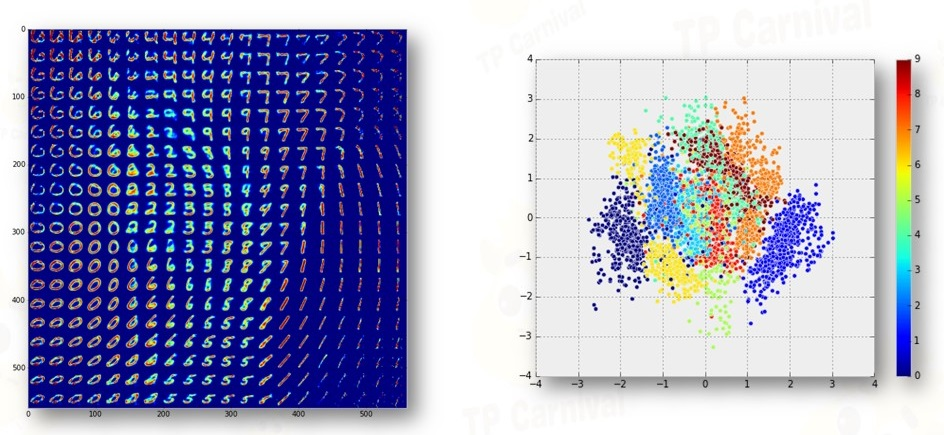
\includegraphics[width=4in]{image/image22.jpg}
\end{center}

\subsection{Make no exception}
这个标题不是说让大家用try catch把exception吞了,这是一视同仁的意思。

卷积网络的核心观点是“一视同仁”,比较适合于二维结构的数据。他的网络结构就像这样,我们先大概浏览一下

\begin{center}
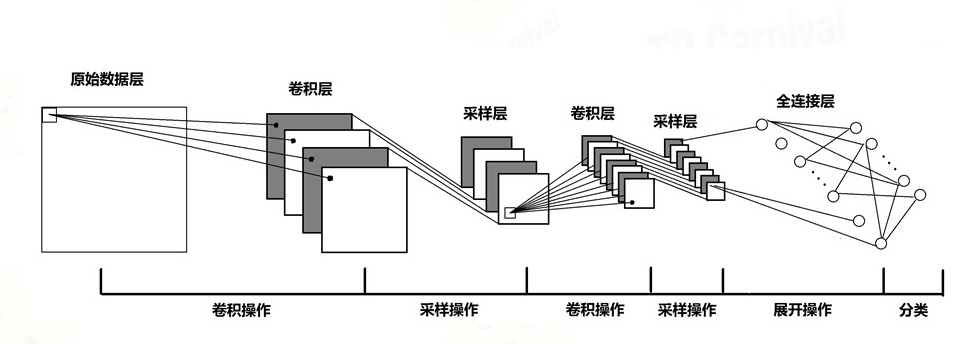
\includegraphics[width=5in]{image/image024.jpg}
\end{center}

以图像为例,我们知道,图像其实就是一个二维矩阵,那么我们就可以通过一个卷积核去卷积这个矩阵,得到一个特征图,如果用多个卷积核,那么就会有多个特征图,接着对卷积的结果进行采样,然后再卷积,再采样,blabla,最后一展开成全连接网络,一个卷积网络就完成了。

那么什么是卷积呢?这个过程就好像这张动图一样(PPT里是动图),固定的卷积核扫过原始的图像,就会扫出一张特征图。
\begin{center}
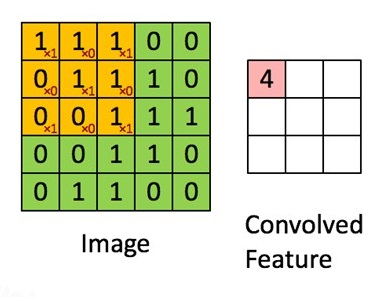
\includegraphics[width=2in]{image/image0250.jpg}
\end{center}
透视图的角度就像这样,卷积核与原始图像对应的位置相乘相加,得到了特征层的一个节点。
\begin{center}
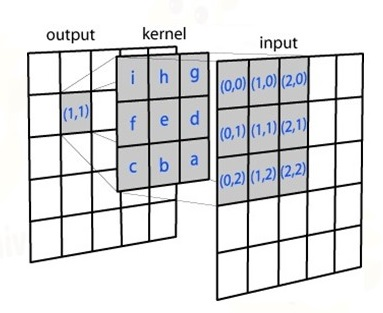
\includegraphics[width=2in]{image/image0251.jpg}
\end{center}

而采样,其实就是取局部小范围内的平均或者最大值。

实际上,你可以将卷积看做是滤波,就像这里,原始RGB三色通道的通道,通过卷积后,我们可以看到,卷积层得到的结果是飞机的机身、翅膀、尾翼,而环境的背景色都不见了,这个过程就像滤波一样,将没用的信息过滤掉,提取出有用的信息。

\begin{center}
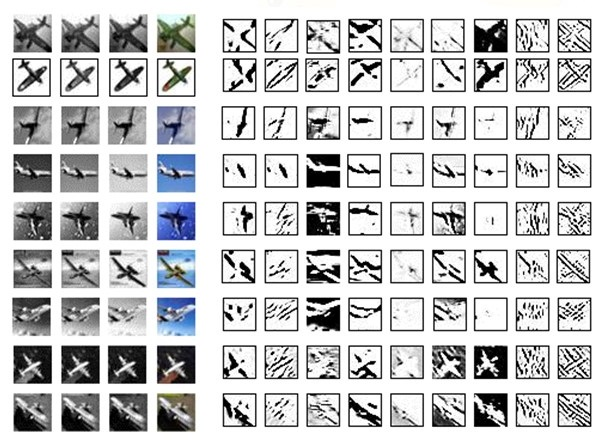
\includegraphics[width=5in]{image/image026.jpg}
\end{center}

\subsection{Experience is the father of wisdom and memory the mother}
虽然卷积网络也可以用来建立时序模型,但受限于卷积核的大小,如果你要建立一个长时序模型,循环神经网络会是一个更好的选择。

\begin{center}
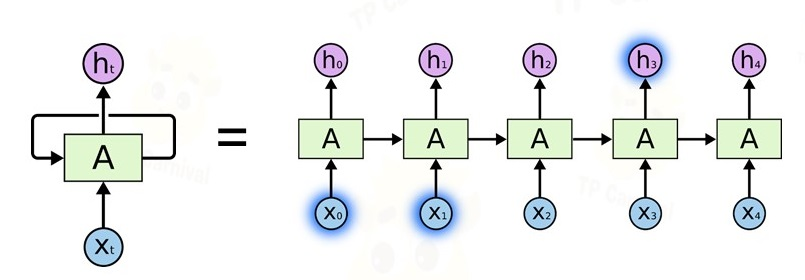
\includegraphics[width=3.5in]{image/image028.jpg}
\end{center}

与之前的两种神经网络不同的是,RNN中允许层内的连接,并且输入和输出都是时间序列。这种结构允许你当前的输出依赖于很久以前的输入。

RNN比较流行的一种结构是LSTM,就像人一样,我们总会忘记东西,这种网络引入了遗忘的概念,他的输出是由当前的输入和经过遗忘后的历史一起组合得到的。构型就像是这样
\begin{center}
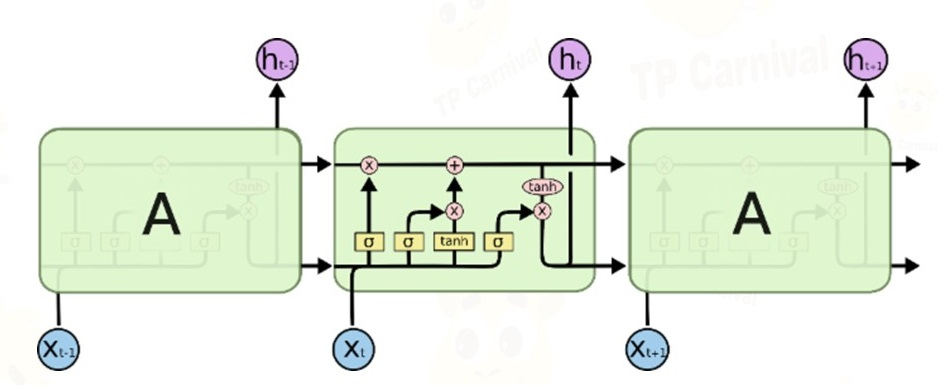
\includegraphics[width=3.5in]{image/image029.jpg}
\end{center}

下面我们将它拆分了介绍,每一个LSTM的节点等同于一个细胞,每个细胞会有自己的状态。一条传送带横穿过去,将细胞状态从上一个细胞传输到下一个细胞,在这根直线上,只会进行线性变换
\begin{center}
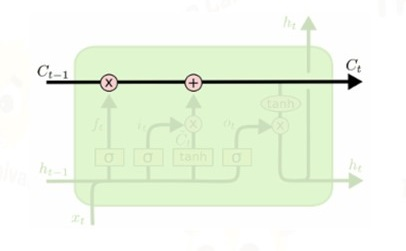
\includegraphics[width=2.2in]{image/image030.jpg}
\end{center}

这条传送带一定走得通吗?不一定,有一个遗忘开关控制着它,这个遗忘开关由上一次的输出和这一次的输入共同决定了这条传送带的口子开多少,1就是全开,0就是全关。
\begin{center}
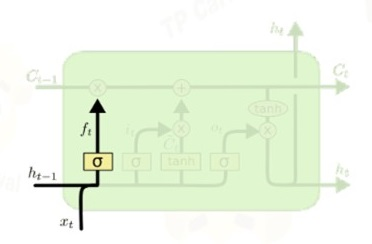
\includegraphics[width=2.2in]{image/image031.jpg}
\end{center}


好,祖传的细胞状态我们得到了,现在考虑当前这一代的细胞状态,我们会选取xt经过一个反正切映射后的一个状态作为新的细胞状态,映射后的xt有这么多个状态,选哪一个呢?这时候就是经过这个sigmoid门来决定选哪一个了。
\begin{center}
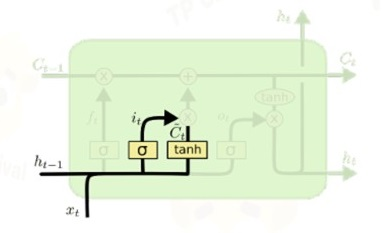
\includegraphics[width=2.2in]{image/image032.jpg}
\end{center}


他们选取后的结果,与祖传的结果一合并,就得到了这个细胞的细胞状态
\begin{center}
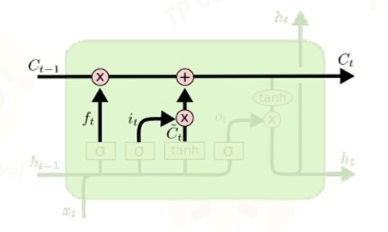
\includegraphics[width=2.2in]{image/image033.jpg}
\end{center}


然后就是这一代的输出值啦,他等于上一个输出值和这个细胞状态的的融合,你看,这两个一加,诶,ht出来了
\begin{center}
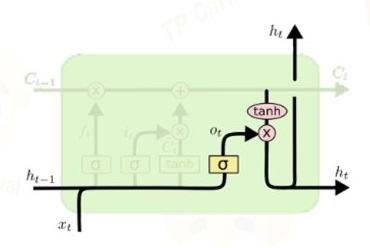
\includegraphics[width=2.2in]{image/image034.jpg}
\end{center}


\subsection{R U crazy?}
当我第一次知道MSRA的何恺明(没错,就是我们隔壁楼的...)建了一个千层级别的神经网络时,我的第一反应就像站在舞台上的雷军,“R..R...R..U..OK?”,但我浏览一下他们的idea后简直惊呆了,整个idea倒也不是很复杂,虽然它叫做残差网络,但我答应过大家,我尽可能的不会再文章中出现数学公式,所以这里我们会从非数学的角度上切入这种结构。

先引入一个奇怪的现象,搞过深层网络的同学做实验的时候应该都会遇到这个现象:随着你网络的加深,性能并不会提升,反而会下降,这个问题看起来不像是因为梯度消失而引起的,因为你的网络也确实收敛了。这就会出现一个悖论了,深层网络理论上是不应该比浅层网络差的,为什么呢?假定一个是3层网络,一个是10层网络,那在10层网络中,我完全可以前3层的参数与那个三层网络的一模一样,而后7层的网络直接做等值映射,也就是后7层直接将第三层的输出不经任何处理的提取出来,这就等价于3层网络了,所以理论上是不应该比3层网络差的。

而ResNet就是基于这么一个思路,既然你后7层可能会给我捣乱,那我就建一条高速公路,直接跳过你,从第三层直接跳到最后一层,这完全是可行的对吧。这就是ResNet最重要的思路,建茫茫多的高速公路,这些高速公路分别可以跳过任何一层,就像下面这幅图一样。

\begin{center}
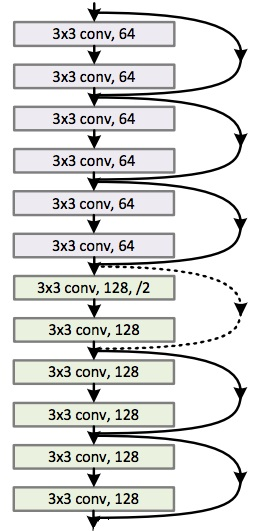
\includegraphics[width=1in]{image/resnet.jpg}
\end{center}

得益于这些高速公路,梯度消失问题也被解决了,因为误差可以走高速快速地返回到第一层,而这种结构可以把神经网络建得非常深,可以想象接下来的时间里,学术界会灌一堆巨型网络(非贬义),或许最大的赢家是Nvidia的老黄。








\section{Welcome back to the land of reality}
欢迎回到肮脏的工业数据。在此之前,容我先介绍一下我们的业务流程。

首先介绍下我们的产品叫“拿去花”,跟我念,“趣拿拿去趣拿拿去趣拿拿去花”,好经过一番洗脑现在大家印象深刻了。我们的产品,类似信用卡的功能,用户在购买机票酒店等产品时,可以选择拿去花给他的额度进行支付而不是信用卡或借记卡,等一个月后他再回来还款或者将这个账单分期还款,当然,跟信用卡一样,分期很有可能会收手续费,这也是我们一个收入来源。

\begin{center}
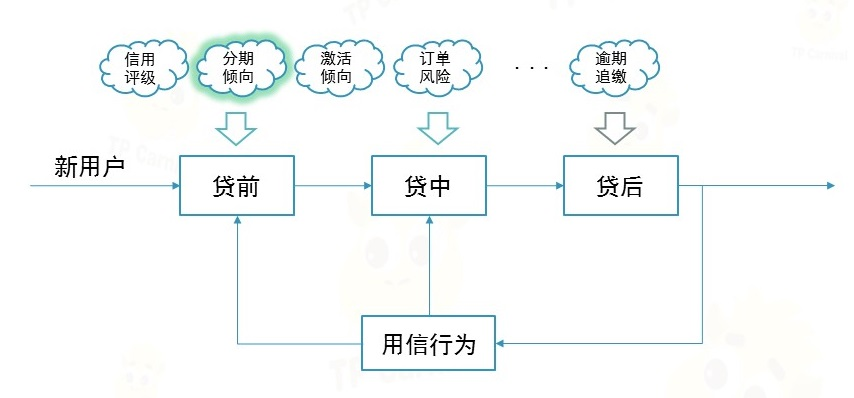
\includegraphics[width=4in]{image/image24.jpg}
\end{center}

那么对于一个用户而言,他的生命周期经过哪些阶段呢?在激活拿去花前,他首先会经过我们贷前的一系列系统的审核,比如信用评级,也就是评估他以后会不会借钱不还,如果说他很有可能借钱不还,那么我们可能会拒绝给他提供信用支付功能。

分期倾向,也就是预测他激活后会不会分期,如果说一个用户,可能因为某种原因,他信用评级不是特别好,但他分期意愿很高,那么我们也有可能允许他开通拿去花,毕竟高风险有高回报嘛。激活倾向,也就是预测用户会不会激活拿去花,如果他倾向很高的话,我们就可能给他推送消息说,爸爸,快来激活拿去花吧。

一旦一个用户激活拿去花,就会进入到贷中阶段,这个阶段订单风险等一系列的贷中模型开始工作。也就是当一个用户下单时,如果模型预测说这很有可能是一笔盗刷行为,那么这笔订单就不允许使用拿去花支付。最后,用户进入贷后阶段,假如一个用户到了本应还款的日子没有还款,并且超出了一定天数,那么逾期追缴模型就开始工作。

整个过程中,积累的用户用信历史会反馈回贷前、贷中、贷后三个阶段的模型,形成一个闭环控制系统,让模型能通过迭代不断地提升精度。而在这么多的模型里面,使用了深度学习的模型是用户分期预测模型,也就是预测一个用户会不会分期。

为什么会在分期模型里用深度学习呢?我们先稍微跑一下题,先讨论一下深度学习和大数据间的关系。
\subsection{Deep Learning and Big Data}
如果将深度学习比喻成东风快递,使命必达,精准定位,货到付款,概不退货。那么大数据就相当于他的燃料,也就是石油。

\begin{center}
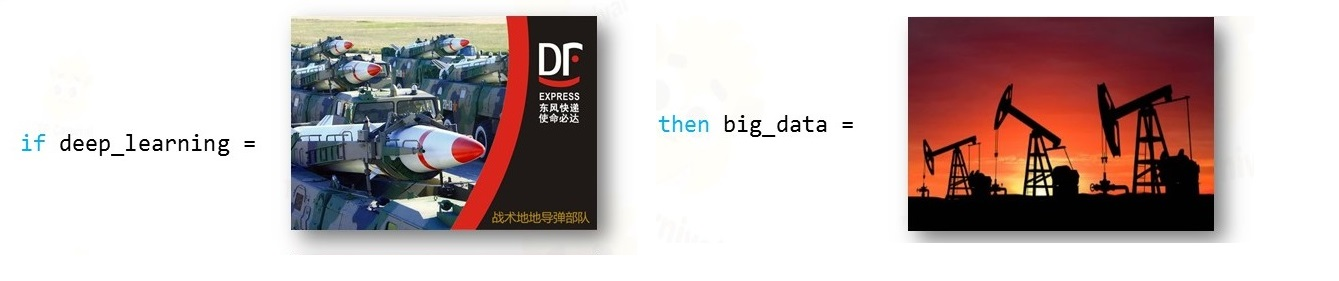
\includegraphics[width=5in]{image/image25.jpg}
\end{center}

由于深度神经网络的参数规模一般较大,这样就VC维就很大了,你需要燃烧掉大量的数据,才能使得你的模型达到比较好的效果。曾经不少朋友会咨询我,锦秀啊,我现在有两千个样本,我可不可以上深度学习啊?这时候我的建议一般都是:如果你要用深度学习,那么你应该先积累数据。这里有一个参考,对于简单的问题,无论你有小规模的或大规模的数据集,都是很简单的一件事。但对于复杂的问题,如果你只有很少的样本,那么我只能说,巧妇难为无米之炊。而如果你有很大的数据集,那么就可以尝试一下深度学习。



我们之所以在分期预测上使用深度学习,是因为分期用户还是挺多的,目前量级大约是几十万,当然随着业务井喷式的发展,这个数量也在快速的增长中,这个量级的样本就可以尝试使用深度学习了。

\subsection{PU-Learning}
工业数据和学术数据一个很大的不同在于,学术数据有很多都是有人维护的,打了标签的数据,比如LeCun等人维护的MNIST,Alex Krizhevsky等人维护的CIFAR-10,以及Feifei等人维护的ImageNet等等。

我不禁想起了我的一个朋友,他们的实验室平时闲来无事就发下兼职广告,有偿的找点学生给他们标注数据啥的,我仿佛看到了发家致富的路子,等下次经济大萧条的时候我就去西二旗摆个地摊让大家都来标注数据为科学献身啥的。严肃,这是一件很严肃的事情,毕竟我们的祖师爷维纳说过,“没有哪台机器比人更牛逼”。这个在机器学习上也是有方向的,叫做“Human Computation”,俗称人肉计算,哈哈哈哈哈哈艾玛不行了我要出去笑一会。

\begin{center}
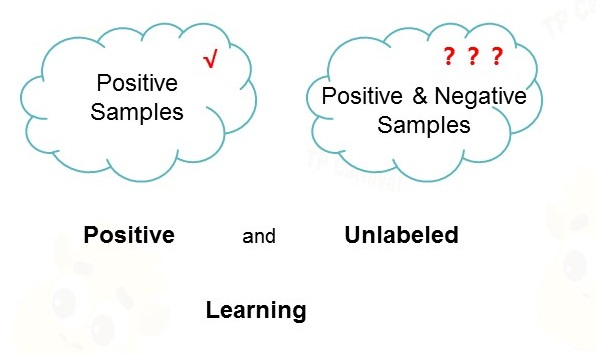
\includegraphics[width=2.5in]{image/image260.jpg}
\end{center}

工业数据中,很多情况下,我们的数据是无标签的,或者有一部分有标签,另一部分没标签,即正负样本都混杂在里面了,这就是所谓的Positive and Unlabeled Learning(PU-Learning)。关于PU-Learning,学术上讨论的不少,但是看起来就觉得很麻烦,而且还不一定在自己的场景中使用。所以我们就不介绍了,我们主要介绍两种简单粗暴的方法。

第一种是所谓的表现期。在分期预测这个任务中,对于分期的用户,毫无疑问,一旦他分期了,那么他的标签就是分期,问题是,不分期的用户,他的标签就是不分期吗?并不是,一个用户不分期,只能说明他现在不分期,并不代表他以后不分期。怎么解决?我们观察了用户激活后的分期情况

\begin{center}
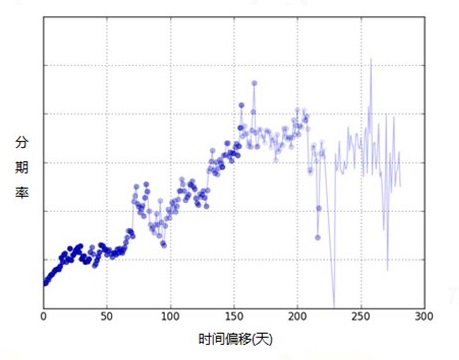
\includegraphics[width=2.5in]{image/image261.jpg}
\end{center}

在这个图中,x轴代表的是时间偏移,y轴代表的是分期率,这个图的含义是,x天前激活的用户,他们的分期率是多少。比如这个点代表一个月前激活的用户他们的激活率是多少。

那么我们可以发现,当x大于120后,分期率是稳定的,也就是说一旦一个用户激活了120天,他还不分期,那他以后也不大可能会分期了。所以我们把激活了120天还不分期的用户打上不分期的标签。

但是120天就是合理的吗?凭什么说我120天不分期以后就不分期?确实,如果我们将时间调长一些,假设200天,这样的话标签会更准,但是这样留下来的样本就会更少。我们选取120天的原因是这个时间点刚好是的正负样本位于均衡状态。

另外一种方法,叫做滚动率。例如在信用评级这个任务中,你怎么定义一个样本为坏样本?逾期一天不还就算作坏样本了吗?显然不行,我忘记还而已,你凭什么就说我是坏用户?那我定义逾期多少天才算作坏用户?这就可以采用滚动率的概念。也就是说,一个用户逾期了,那他就相当于往坏用户方向滚动,一旦他还钱了,就相当于往好用户滚动。那么我们就可以测试,各个逾期天数下会还款的用户比例,从而可以知道,一旦用户逾期了t天,他还会还钱的可能有多大,这样你就可以下断言说,一个用户一旦逾期超过t天,那他还钱的概率我无法接受,认为他是坏用户,也就是认为他以后再也不会滚回来了。

想像一下前面这个圆圆的东西是你前男友,你轻轻踹他一脚,嘿他往前滚一会又滚回来了,但如果你卯足了劲踹他一脚,他就咕噜咕噜往前滚再也不回来了,看着就觉得好玩,不过前男友这种东西,虽然活着,但已经死了,管他做啥呢?
\subsection{Bool Unit}
与图像或语音中的任务不同的是,在那些任务中,特征是不需要经过太多预处理的,可以直接将像素点作为神经元扔进去.但是金融数据里,每个特征都是有自己的含义的,各自的纲量也不同.比如,某个节点代表的是机票消费金额,他的量级可能是万,而另一个节点代表机票订单数,量级可能是十几二十这样.那么对于这种数据我们怎么处理呢?我们的方法是将他们离散化成01的布尔节点.假设,我们用10个节点来表示消费金额,如果用户的金额小于1000,那么第一个节点为1,其他为0,如果为2000,那么第二个节点为1,其他为0,以此类推.

这种预处理会有什么好处呢?首先他降低了对异常值的敏感度,想想一下,如果因为某种原因导致某个用户机票消费金额是几百万,倘若用的是连续值的神经元,那完了,这就可能输出一个非常大的值.而采用布尔节点就不会发生这种情况,因为几百万仅仅只是激活了最大档的神经元.

另一方面,假设决策边界是 $ y=x^2 $, 如果使用连续值,训练出来的决策边界可能是$ y=kx+b $,这样就会有部分的样本会被错误分类.

\begin{center}
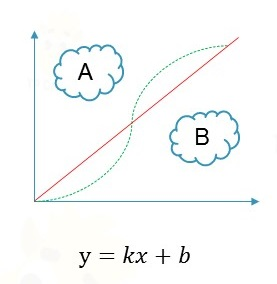
\includegraphics[width=1.5in]{image/image271.jpg}
\end{center}

但如果我们将x离散化成三段,那么决策边界就是一个分段函数,也就是说,当x位于$x_1$这段时,y等于$y_1$,位于$x_2$这个区间时y等于$y_2$.
\begin{center}
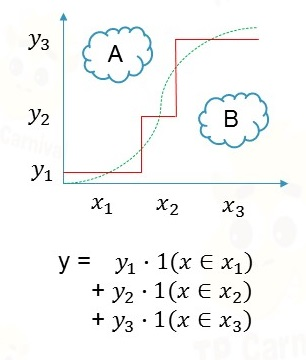
\includegraphics[width=1.5in]{image/image272.jpg}
\end{center}

如果我们将x分得更细,那么就可以更精确地逼近决策面.

\begin{center}
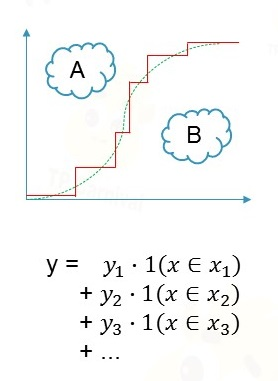
\includegraphics[width=1.5in]{image/image273.jpg}
\end{center}

因为我们是消费型公司,所以我们有的数据也会偏向消费数据, 例如用户的机票酒店等订单信息,这些信息再结合上支付信息以及他的一些账号信息,像注册时长等,总共提取了100多个特征,这些特征经过布尔化后,得到了我们网络输入层中700多个结点.

上面的都是骗你们的,我们之所以布尔化的真正原因是RBM只支持伯努利节点...

\subsection{Compute Capability}
最后一个问题是计算性能问题.由于深度学习的样本大,同时网络参数多,cpu就不太适合了,因此我们采用的是GPU,也就是显卡,来计算。如果把cpu比作python,瑞士军刀型语言,啥都能干,那么gpu就好比PHP,虽然功能单一,有时用不好会伤到自己,但是我们人多啊。

\begin{center}
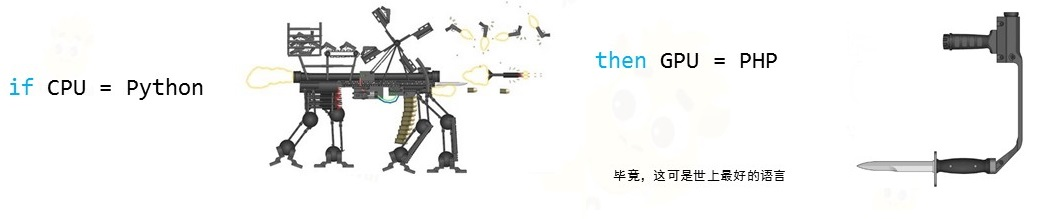
\includegraphics[width=5in]{image/image29.jpg}
\end{center}

比如一个三维矩阵,我要将每个元素都加1,那么cpu就要跑一个循环了,而对于GPU,他可以并行的在每个元素上+1s,但是GPU也不是万能的,它只能实现一些简单的逻辑功能,像加减乘除之类的,就像一名小学生,如果你让他去做一些很复杂的逻辑,就好比让一名小学生算一个定积分,他就不那么擅长了.

\subsection{Our Choice}
我们采取的计算框架是tensorflow和gnumpy,也就是gpu版的numpy,最后训练一个6层的神经网络,其中,前五层是RBM结构,最后一层是softmax结构。倒数两层采用了dropout惩罚。

\begin{center}
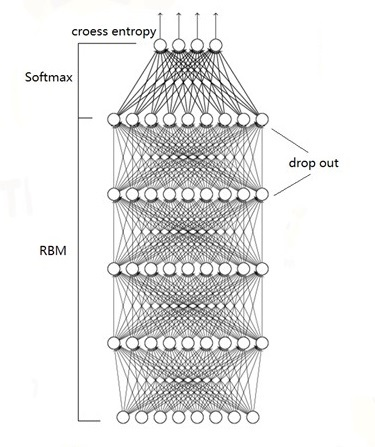
\includegraphics[width=2in]{image/image30.jpg}
\end{center}

为什么层数设定为6而不是更深呢?一方面,我们的数据量只能够支持到6层网络,更深的网络性能就开始下降了,当然,网络性能下降也有很大的原因是网络结构问题,我们最近也在切换残差网络的过程中.

\begin{center}
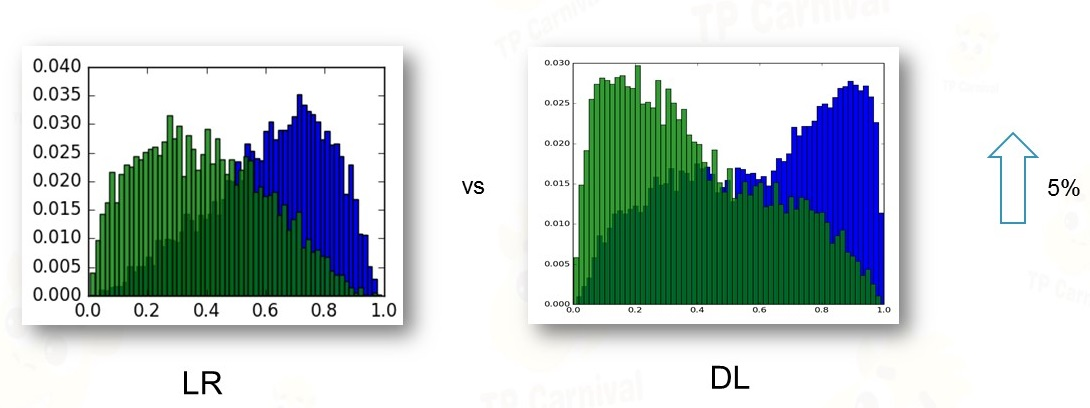
\includegraphics[width=5in]{image/image31.jpg}
\end{center}

相比于传统的分类器,使用了深度学习后,auc大约提升了5个百分点左右,虽然没有像imagenet那样一下子提升20个百分点,但5个百分点总比没有的好嘛。我们可以看到,深度学习训练出来的分类器对正负样本的区分能力会更强一些,也就是说,位于0.5附近的样本会少很多,或者说,ks值更大一些。

为什么我们不用hadoop或者spark呢?因为hadoop这种更倾向于批处理,或者说是比较粗粒度的并行,而在深度学习里面,需要的是细粒度的并行,如果用hadoop之类的话,通讯就是很大问题了。

\subsection{How to use?}
如何使用,或者说你想要用深度学习,应该怎么办?

\begin{center}
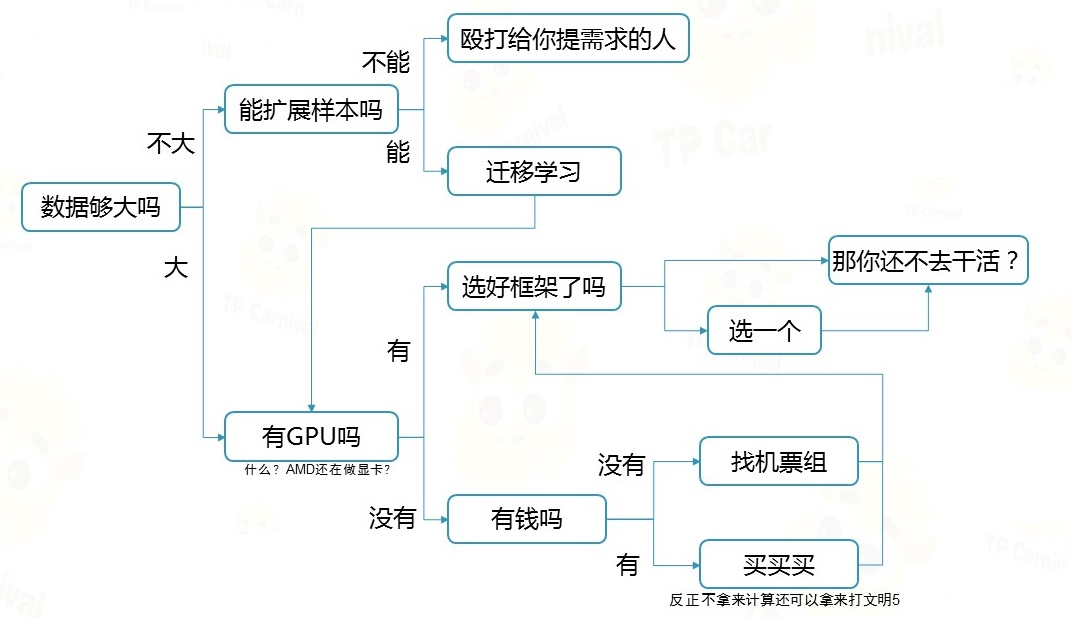
\includegraphics[width=5in]{image/image32.jpg}
\end{center}

首先第一件事,你问一问自己,我的数据是不是足以上深度学习,毕竟你总不能拿大炮来打蚊子吧。那多少算足够呢?有个不太靠谱的个人建议,如果你的数据随便用个啥模型跑跑轻松能到80+左右的正确率,那么10W左右的样本是底线,如果只有70+,那么怎么也得要个几十万样本吧,当然了,样本是越多越好的,你会嫌你银行卡里的余额多吗?并不会。

如果你没有那么多样本,怎么办?那你就问问你自己有没有办法扩展一下样本,例如,如果你在做图像识别,那么将图像镜像一下,嘿,数据量立马就翻倍了,不过你要是说你的图片都是俄罗斯那种对称风格的建筑,那只好节哀了...不过不要紧,你还是可以借助一下搜索引擎来扩展你的样本集的嘛,说道图片检索,我只服百度这位老司机,无论你的关键词是什么总能搜到一些迷の图片。

另一种做法,就是迁移学习了,我们只介绍迁移学习中的一种,也就是样本迁移,比如说,你要做用户的银行卡号识别或者别的数字识别啥的,当然你可以用机器视觉那一套(不管怎样,你还是得要用一些机器视觉的东西的,毕竟识别前你总得提取数字吧),问题来了,你没有那么多银行卡号的数字,怎么办?google上扒?多累啊,而且还吃力不讨好。这时候你可以尝试一下拿MNIST的数据集和你的银行卡号数据集混合在一起做训练,嘿,样本量立马就上去了,不过要注意一下,验证集要用银行卡号的数据,你想想,我做的是银行卡识别,最后MNIST识别再高对我都没啥用啊。

好,我不管你了,我假设你现在有了大数据,接下来就要问问你有没有GPU了,如果你没有GPU,那么就问问你有没有钱,如果你没有钱,\sout{艾玛,我说你这孩子咋啥都没有},那么你可以找机票组的同学,他们有Tesla的GPU,平时有啥深度学习的问题也可以跟他们讨论,毕竟那边的师资更雄厚,\sout{麻烦机票组的同学结算一下广告费}。如果你有钱,毫无疑问当然是买买买,三千预算进卡吧,四路泰坦带回家,\sout{反正最后都是拿来打游戏}。但是要注意,你只能买Nvidia的卡,\sout{什么?AMD还在做显卡},毕竟CUDA要甩OpenCL几条街,而且目前几乎所有的计算框架都是基于CUDA的,买啥型号好呢?建议GTX1080或新架构的Titan,因为内存真的很重要,不过不清楚现在的框架们支持cuda8.0没有,具体的再私聊吧不深究了,毕竟这东西要说起来一匹布那么长。

现在假定你有GPU了,不管你是买的借的偷的反正就是有了,那么你选好计算框架了吗?现在深度学习的计算框架已经很成熟了,像Caffe, MxNet, TensorFlow, Theano, Torch等等一大堆,\sout{应该不会有人直接用CUDA吧},我不禁想起以前还没有这些框架时的那段峥嵘岁月,那时候都是手动写反向传播的,做梯度校验分分钟让你怀疑人生,不过现在的框架已经十分便利了,基本都是走的自动求导,也就是不用自己写反向传播了,简直是懒人的福音。

这么多框架选哪个呢?我的建议是TensorFlow。虽然这东西刚出的时候被MxNet吊打,不过好在TensorFlow是个富二代,人家爸爸可是大名鼎鼎的Google(当然MxNet的爸爸李沐也很牛逼,Parameter Server的作者,我没有说Caffe的贾扬清不牛逼,将来报道上出了偏差我不负责),所以咯,一年时间不到,TensorFlow已经从一只丑小鸭变成了丑大鸭,港真,它的内存管理可以被我黑一辈子...如果你对C++比较熟悉,而做的东西跟图像又比较相关,那么可以选择Caffe。因为目前GPU版的TensorFlow只支持linux,所以如果你无法忍受linux的话,windows下的MxNet也是个不错的选择。gNumpy我十分推荐使用,一个轻量级的GPU版矩阵运算,功能有限,但是很灵活。

现在你有了数据,有了GPU,有了框架,那你还不赶紧干活?

\section{结束语}
这篇文章之所以叫做深度学习防骗指南,是为了让你以后再遇到鼓吹深度学习无所不能的香港记者时,piapia两个大嘴巴子,“我爸爸从小就教育我,有多少人工,就有多少智能”,事了拂衣去,深藏功与名





\end{CJK}
\end{document}

